\begin{figure}
  \centering
  \hspace*{-17mm}
  \begin{tikzpicture}[
    below_label/.style={text width=4.5cm,align=center,inner sep=2pt},
    arrow_label/.style={midway,sloped,inner sep=2pt},
    node distance=1.5
  ]
    \node [base_node, yshift=6, xshift=6] at (0,0) {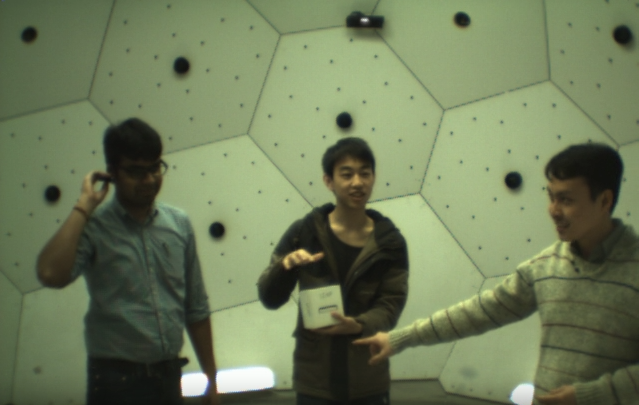
\includegraphics[width=15mm]{figures/examples/example1.png}};
    \node [base_node, yshift=4, xshift=4] at (0,0) {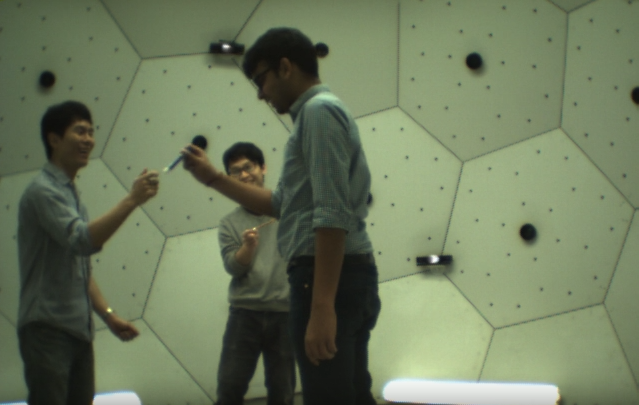
\includegraphics[width=15mm]{figures/examples/example2.png}};
    \node [base_node, yshift=2, xshift=2] at (0,0) {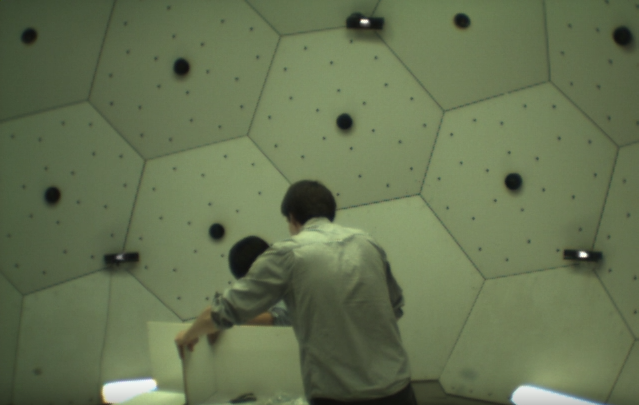
\includegraphics[width=15mm]{figures/examples/example3.png}};
    \node [base_node] (video_box) at (0,0) {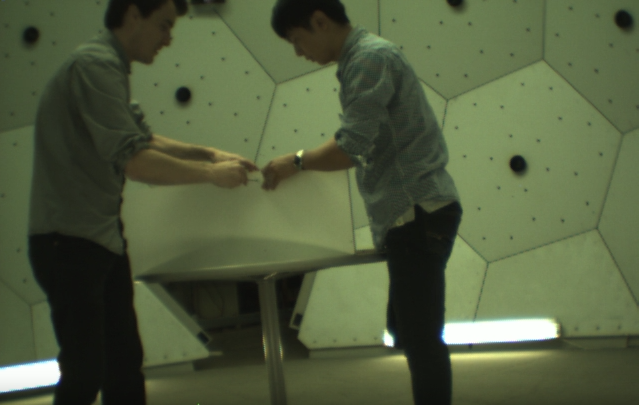
\includegraphics[width=15mm]{figures/examples/example4.png}};
    \node[below_label, below=0 of video_box] (video_label) {Multi-View Videos};

    \node [base_node, right=1.3 of video_box, yshift=6, xshift=6] {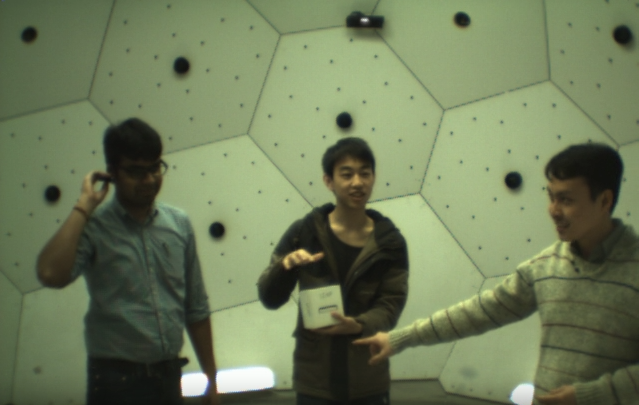
\includegraphics[width=15mm]{figures/examples/example1.png}};
    \node [base_node, right=1.3 of video_box, yshift=4, xshift=4] {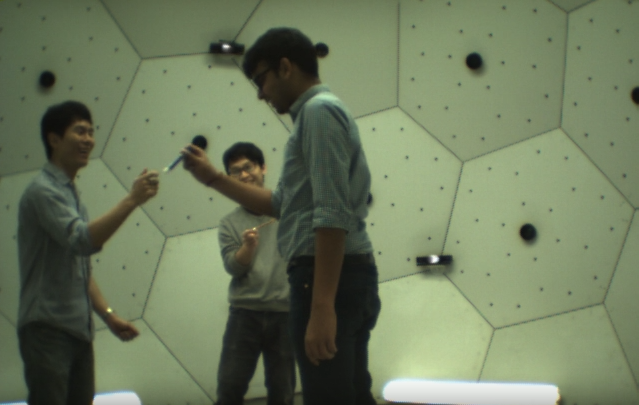
\includegraphics[width=15mm]{figures/examples/example2.png}};
    \node [base_node, right=1.3 of video_box, yshift=2, xshift=2] {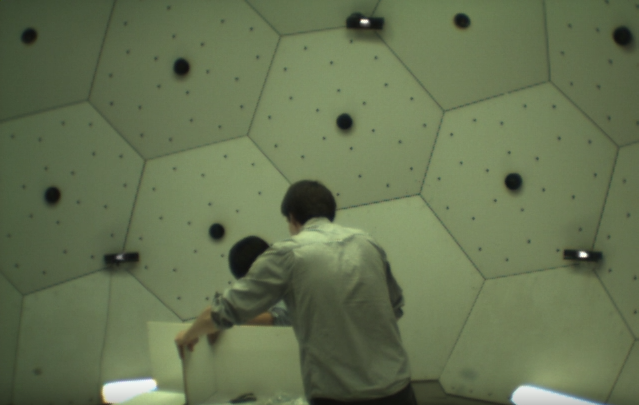
\includegraphics[width=15mm]{figures/examples/example3.png}};
    \node [base_node, right=1.3 of video_box] (detections_box)  {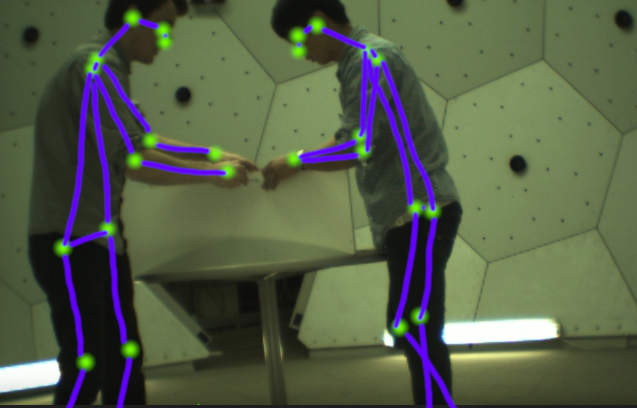
\includegraphics[width=15mm]{figures/examples/example4_pred.png}};
    \node[below_label, below=0 of detections_box] (detections_label) {2D Detections};

    \node[base_node, right=1 of detections_box] (match_box) {
      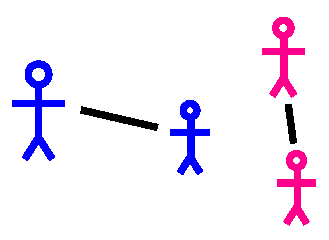
\includegraphics[width=15mm]{figures/match.pdf}
    };
    \node[below_label, below=0 of match_box] (match_label) {Match Detections};

    \node[base_node, above=of $(detections_box.south)!0.5!(match_box.south)$, yshift=30] (predict_box) {
      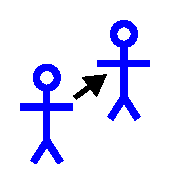
\includegraphics[width=10mm]{figures/predict.pdf}
    };
    \node[below_label, below=0 of predict_box, xshift=-30] (predict_label) {Predict 3D State};

    \node[base_node, above right=of match_box, yshift=-40] (kf_box) {
      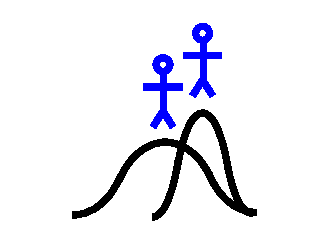
\includegraphics[width=15mm]{figures/update.pdf}
    };
    \node[below_label, above=0 of kf_box] (kf_label) {Kalman Filter Update};

    \node[base_node, below right=of match_box, yshift=40] (tri_box) {
      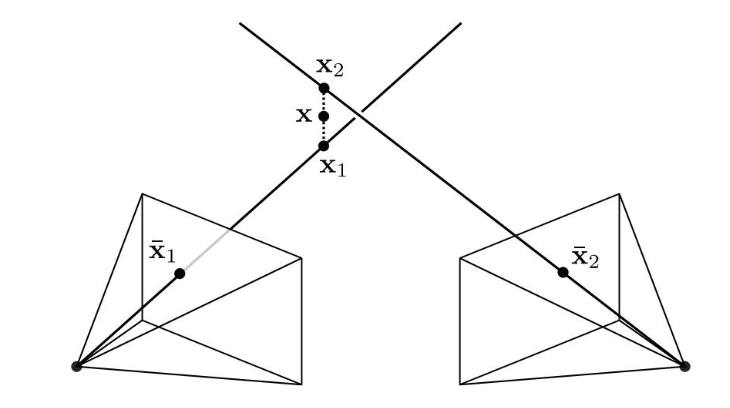
\includegraphics[width=15mm]{figures/triangulate.png}
    };
    \node[below_label, below=0 of tri_box] (tri_label) {Triangulate};

    \node[base_node, right=1 of $(kf_box.east)!0.5!(tri_box.east)$] (merge_box) {
      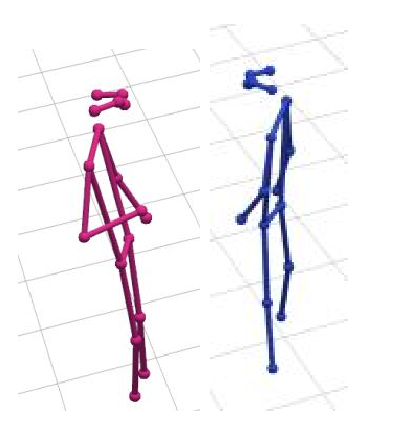
\includegraphics[width=15mm]{figures/merged.pdf}
    };
    \node[below_label, below=0 of merge_box] (merge_label) {Merge Tracks};

    \draw[flow] (video_box) -- (detections_box)
      node[arrow_label, pos=0.5, below] {YOLO};
    \draw[flow] (detections_box) -- (match_box);
    \draw[flow] (predict_box) -- (match_box);

    \draw[flow] (match_box.east) -- (kf_box.west) 
        node[arrow_label, pos=0.5, above] {Old};
    \draw[flow] (match_box.east) -- (tri_box.west) 
        node[arrow_label, pos=0.5, below] {New};

    \draw[flow] (kf_box.east) -- (merge_box.west);
    \draw[flow] (tri_box.east) -- (merge_box.west);

    \draw[flow] (merge_box.north) |- (predict_box.east)
        node[arrow_label, pos=0.2, above] {Repeat};
  \end{tikzpicture}
\end{figure}
